\HeadingLevelB{SGX Physical Memory Organization}
\label{sec:sgx_prm}

% Intel SGX Resource Enumeration Leaves: SDM S 37.7.2
% Interactions with DMA: SDM S 42.10, SGX2 S 6.10

The enclaves' code and data is stored in \textit{Processor Reserved Memory}
(PRM), which is a subset of DRAM that cannot be directly accessed by other
software, including system software and SMM code. The CPU's integrated memory
controllers (\S~\ref{sec:cpu_die}) also reject DMA transfers targeting the PRM,
thus protecting it from access by other peripherals.

% EPC and Management of EPC Pages: SGX2 S 3.5
% Interactions with Memory Configuration: SGX2 S 6.11
% Memory Type Considerations for PRMRR: SGX2 S 6.11.1
% Interactions of PRMRR with Physical Memory Accesses: SGX2 S 6.11.3.1

The PRM is a continuous range of memory whose bounds are configured using a
base and a mask register with the same semantics as a variable memory type
range~(\S~\ref{sec:cacheability_config}). Therefore, the PRM's size must be an
integer power of two, and its start address must be aligned to the same power
of two. Due to these restrictions, checking if an address belongs to the PRM
can be done very cheaply in hardware, using the circuit outlined in
\S~\ref{sec:cacheability_config}.

The SDM does not describe the PRM and the PRM range registers (PRMRR). These
concepts are documented in the SGX
manuals~\cite{intel2013sgxmanual, intel2014sgx2manual} and in one of the SGX
papers~\cite{mckeen2013sgx}. Curiously, although the SDM generally mirrors the
SGX manuals, it lacks most of the sections that mention the PRM.


\HeadingLevelC{The Enclave Page Cache (EPC)}
\label{sec:sgx_epc}

% Enclave Page Cache: SDM S 37.5
% EPC and Management of EPC Pages: SDM S 39.5, S 39.5.1

The contents of enclaves and the associated data structures are stored in the
\textit{Enclave Page Cache} (EPC), which is a subset of the PRM, as shown in
Figure~\ref{fig:sgx_epc}.

\begin{figure}[hbt]
  \centering
  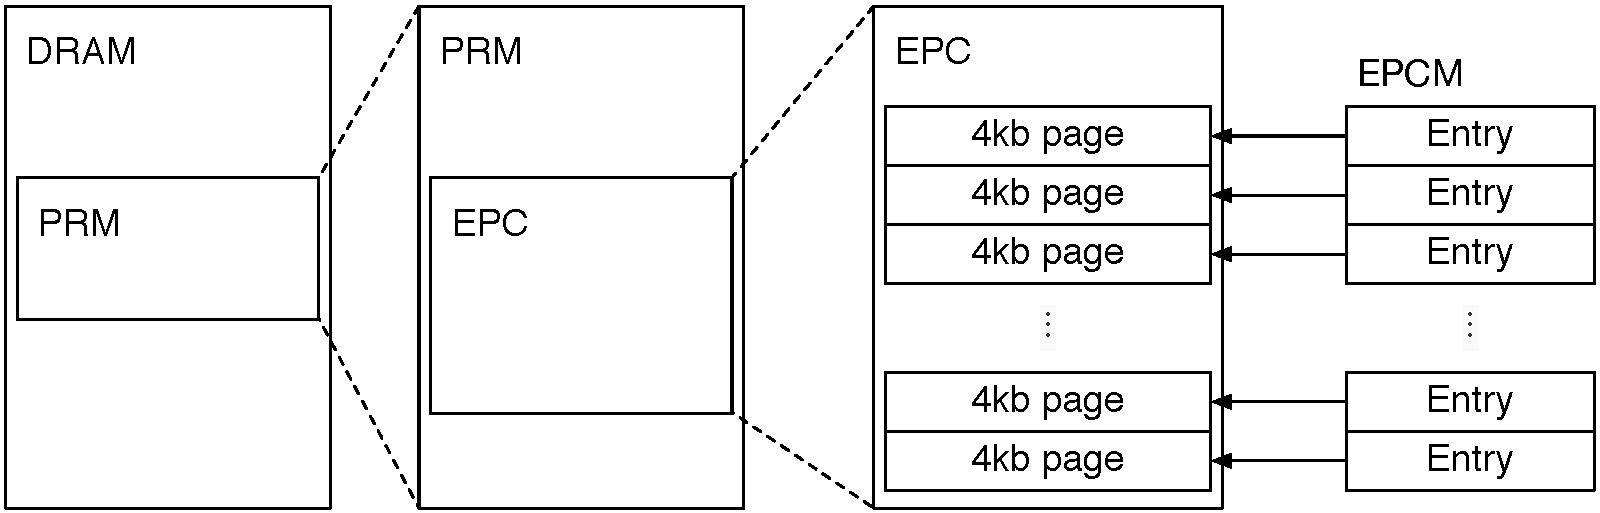
\includegraphics[width=87mm]{figures/sgx_epc.pdf}
  \caption{
    Enclave data is stored into the EPC, which is a subset of the PRM. The
    PRM is a contiguous range of DRAM that cannot be accessed by system
    software or peripherals.
  }
  \label{fig:sgx_epc}
\end{figure}

The SGX design supports having multiple enclaves on a system at the same time,
which is a necessity in multi-process environments. This is achieved by having
the EPC split into 4~KB pages that can be assigned to different enclaves. The
EPC uses the same page size as the architecture's address translation feature
(\S~\ref{sec:paging}). This is not a coincidence, as future sections will
reveal that the SGX implementation is tightly coupled with the address
translation implementation.

The EPC is managed by the same system software that manages the rest of the
computer's physical memory. The system software, which can be a hypervisor or
an OS kernel, uses SGX instructions to allocate unused pages to enclaves, and
to free previously allocated EPC pages. The system software is expected to
expose enclave creation and management services to application software.

Non-enclave software cannot directly access the EPC, as it is contained in the
PRM. This restriction plays a key role in SGX's enclave isolation guarantees,
but creates an obstacle when the system software needs to load the initial code
and data into a newly created enclave. The SGX design solves this problem by
having the instructions that allocate an EPC page to an enclave also initialize
the page. Most EPC pages are initialized by copying data from a non-PRM memory
page.


\HeadingLevelC{The Enclave Page Cache Map (EPCM)}
\label{sec:sgx_epcm}

% Enclave Page Cache Map (EPCM): SDM S 37.5.1, SDM S 38.19
% SECINFO.FLAGS: SDM S 38.11.1
% PAGE_TYPE Field Definition: SDM S 38.11.2

The SGX design expects the system software to allocate the EPC pages to
enclaves. However, as the system software is not trusted, SGX processors check
the correctness of the system software's allocation decisions, and refuse to
perform any action that would compromise SGX's security guarantees. For
example, if the system software attempts to allocate the same EPC page to two
enclaves, the SGX instruction used to perform the allocation will fail.

In order to perform its security checks, SGX records some information about the
system software's allocation decisions for each EPC page in the
\textit{Enclave Page Cache Map}~(EPCM). The EPCM is an array with one entry
per EPC page, so computing the address of a page's EPCM entry only requires a
bitwise shift operation and an addition.

The EPCM's contents is only used by SGX's security checks. Under normal
operation, the EPCM does not generate any software-visible behavior, and
enclave authors and system software developers can mostly ignore it.
Therefore, the SDM only describes the EPCM at a very high level, listing the
information contained within and noting that the EPCM is ``trusted memory''.
The SDM does not disclose the storage medium or memory layout used by the EPCM.

The EPCM uses the information in Table~\ref{fig:sgx_epcm_ownership_fields} to
track the ownership of each EPC page. We defer a full discussion of the EPCM to
a later section, because its contents is intimately coupled with all of SGX's
features, which will be described over the next few sections.

\begin{table}[hbt]
  \centering
  \begin{tabularx}{\columnwidth}{| l | r | X |}
  \hline
  \textbf{Field} & \textbf{Bits} & \textbf{Description}\\
  \hline
  VALID & 1 & 0 for un-allocated EPC pages \\
  \hline
  PT & 8 & page type \\
  \hline
  ENCLAVESECS &  & identifies the enclave owning the page \\
  \hline
  \end{tabularx}
  \caption{
    The fields in an EPCM entry that track the ownership of pages.
  }
  \label{fig:sgx_epcm_ownership_fields}
\end{table}

The SGX instructions that allocate an EPC page set the VALID bit of the
corresponding EPCM entry to 1, and refuse to operate on EPC pages whose VALID
bit is already set.

The instruction used to allocate an EPC page also determines the page's
intended usage, which is recorded in the \textit{page type} (PT) field of the
corresponding EPCM entry. The pages that store an enclave's code and data are
considered to have a \textit{regular} type (PT\_REG in the SDM). The pages
dedicated to the storage of SGX's supporting data structures are tagged with
special types. For example, the PT\_SECS type identifies pages that hold SGX
Enclave Control Structures, which will be described in the following section.
The other EPC page types will be described in future sections.

Last, a page's EPCM entry also identifies the enclave that owns the EPC page.
This information is used by the mechanisms that enforce SGX's isolation
guarantees to prevent an enclave from accessing another enclave's private
information. As the EPCM identifies a single owning enclave for each EPC page,
it is impossible for enclaves to communicate via shared memory using EPC pages.
Fortunately, enclaves can share untrusted non-EPC memory, as will be discussed
in \S~\ref{sec:sgx_paging}.


\HeadingLevelC{The SGX Enclave Control Structure (SECS)}
\label{sec:sgx_secs}

% Data Structures and Enclave Operation: SDM S 37.4
% SGX Enclave Control Structure (SECS): SDM S 38.7, S 38.7.1

SGX stores per-enclave metadata in a
\textit{SGX Enclave Control Structure}~(SECS) associated with each enclave.
Each SECS is stored in a dedicated EPC page with the page type PT\_SECS. These
pages are not intended to be mapped into any enclave's address space, and are
exclusively used by the CPU's SGX implementation.

% Constructing an Enclave: SDM S 39.1
% ECREATE: SDM S 39.1.1, S 41.3
% Implicit vs. Explicit accesses: SDM S 38.5.3
% Implicit accesses: SDM S 38.5.3.2

An enclave's identity is almost synonymous to its SECS. The first step in
bringing an enclave to life allocates an EPC page to serve as the enclave's
SECS, and the last step in destroying an enclave deallocates the page holding
its SECS. The EPCM entry field identifying the enclave that owns an EPC page
points to the enclave's SECS. The system software uses the virtual address of
an enclave's SECS to identify the enclave when invoking SGX instructions.

% Access Control Requirements: SDM S 38.3

All SGX instructions take virtual addresses as their inputs. Given that SGX
instructions use SECS addresses to identify enclaves, the system software must
create entries in its page tables pointing to the SECS of the enclaves it
manages. However, the system software cannot access any SECS page, as these
pages are stored in the PRM. SECS pages are not intended to be mapped inside
their enclaves' virtual address spaces, and SGX-enabled processors explicitly
prevent enclave code from accessing SECS pages.

% SGX Enclave Control Structure (SECS): SDM S 38.7, S 38.7.1

This seemingly arbitrary limitation is in place so that the SGX implementation
can store sensitive information in the SECS, and be able to assume that no
potentially malicious software will access that information. For example, the
SDM states that each enclave's measurement is stored in its SECS. If software
would be able to modify an enclave's measurement, SGX's software attestation
scheme would provide no security assurances.

The SECS is strongly coupled with many of SGX's features. Therefore, the pieces
of information that make up the SECS will be gradually introduced as the
different aspects of SGX are described.
